\section{Ant Build}

Ant is used as the build tool for Kieker. %
The important ant targets included in the \texttt{build.xml} file are:

\begin{itemize}
\item \textbf{build-all:} This is the default target that compiles the Kieker %
artifacts and creates the following jar/war files in the \texttt{dist/} directory:
\begin{compactitem}
\item \texttt{kieker-analysis-1.5-trunk.jar} 
\item \texttt{kieker-common-1.5-trunk.jar}
\item \texttt{kieker-monitoring-1.5-trunk.jar}
\item \texttt{kieker-monitoring-servlet-1.5-trunk.war}
\item \texttt{kieker-tools-1.5-trunk.jar}
\end{compactitem}
\item \textbf{javadoc:} Executes Javadoc to create the API documentation in HTML. %
After a successful execution, open \texttt{build/javadoc/index.html} in your %
Web browser.
\item \textbf{run-tests-junit:} Runs the JUnit tests and creates a HTML report %
of the results. 
\item \textbf{run-test$[$s$]$-*:} Additional regression tests mostly employing %
AspectJ for instrumentation. 
\item \textbf{release:} Creates the following Kieker release files in the %
\texttt{dist/release/} directory:
\begin{compactitem}
\item \texttt{kieker-<version>\_javadoc.(zip|tar.gz)}
\item \texttt{kieker-<version>\_binaries.(zip|tar.gz)}
\item \texttt{kieker-<version>\_sources.(zip|tar.gz)}
\item \texttt{kieker-<version>\_examples-JPetStoreExample.(zip|tar.gz)}
\item \texttt{kieker-<version>\_examples-MySimpleKiekerAspectJExample.(zip|tar.gz)}
\item \texttt{kieker-<version>\_examples-MySimpleKiekerJMSExample.(zip|tar.gz)}
\item \texttt{kieker-<version>\_examples-OverheadEvaluationMicrobenchmark.(zip|tar.gz)}
\end{compactitem}
\end{itemize}

\section{IDE-Specific Project Configuration}

This section describes how to create a project for developing with the 
Kieker sources in different IDEs.

\subsection{Netbeans}

You create a Netbeans project for the Kieker trunk as follows:

\begin{compactenum}
\item File->New Project\ldots and select \textit{Java Free-Form Project} and 
follow the wizard and answer the dialogs as follows:

\begin{compactenum}
\item \textbf{Name and Location (Fig.~\ref{fig:nb:location}):} %

Select Kieker's \texttt{trunk/} directory as the project location and th wizard will %
complete the missing information based on the existing \texttt{build.xml} file.

\begin{figure}[H]\centering
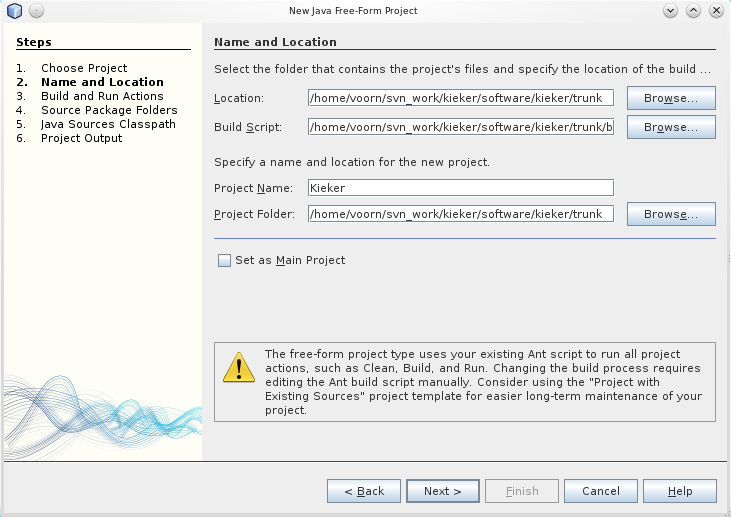
\includegraphics[scale=0.4]{figures/netbeans-NameAndLocation}
\caption{}
\label{fig:nb:location}
\end{figure}

\item \textbf{Build and Run Actions (Fig.~\ref{fig:nb:buildRun}):} %

Complete the information as shown in Fig.~\ref{fig:nb:buildRun}.

\begin{figure}[H]\centering
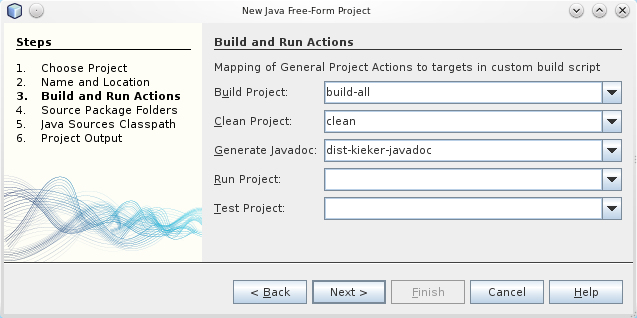
\includegraphics[scale=0.4]{figures/netbeans-BuildAndRun}
\caption{}
\label{fig:nb:buildRun}
\end{figure}

\item \textbf{Source Package Folders (Fig.~\ref{fig:nb:sourcePackageFolders}):} %

\textbf{Add} alls subdirectories of \texttt{src/} and all subdirectories of %
\texttt{ test/} (except for \texttt{test/META-INF/}) to the list of %
\textit{Source Package Folders}. %
\textbf{Remove all \textit{Test Package Folders} entries.}

\begin{figure}[H]\centering
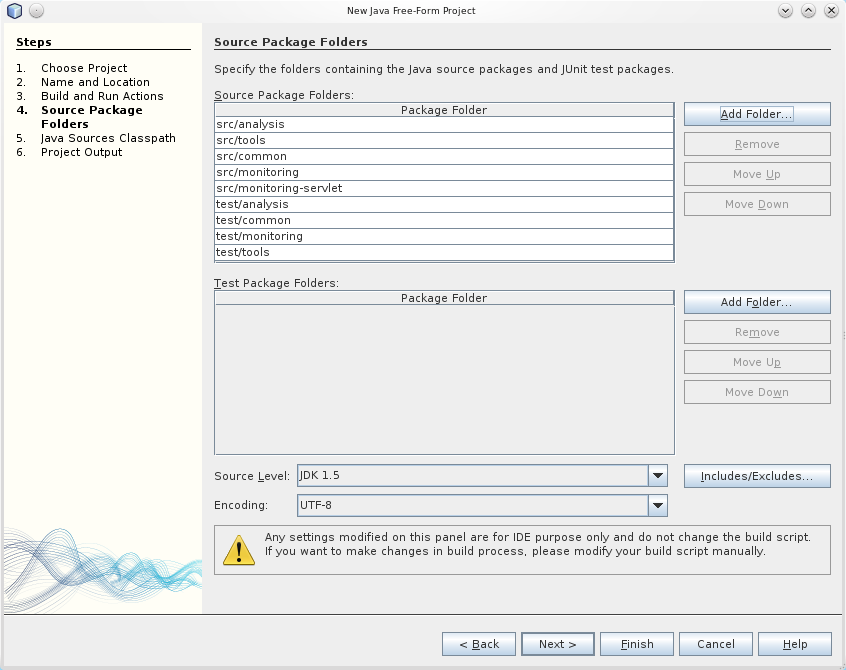
\includegraphics[scale=0.4]{figures/netbeans-SourcePackageFolders}
\caption{}
\label{fig:nb:sourcePackageFolders}
\end{figure}

\item \textbf{Java Sources Classpath (Fig.~\ref{fig:nb:sourcesclasspath}):} %

\textbf{\underline{Un}check} the option \textit{Separate Classpath for Each Source Package Folder} and %
\textbf{add} all .jar files included in the \texttt{lib/} directory.

\begin{figure}[H]\centering
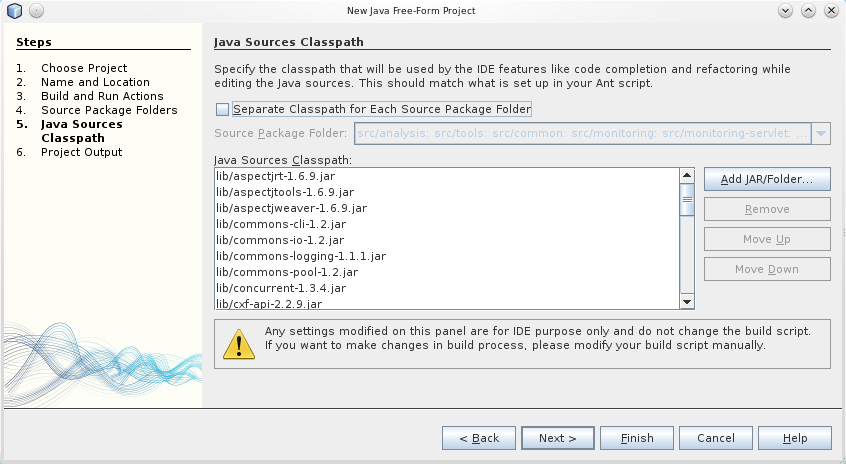
\includegraphics[scale=0.4]{figures/netbeans-SourcesClasspath}
\caption{}
\label{fig:nb:sourcesclasspath}
\end{figure}

\item \textbf{Project Output (Fig.~\ref{fig:nb:projectOutput})} %

Simply skip this dialog without any changes and finish the wizard by clicking %
on the \textbf{Finish} button.

\begin{figure}[H]\centering
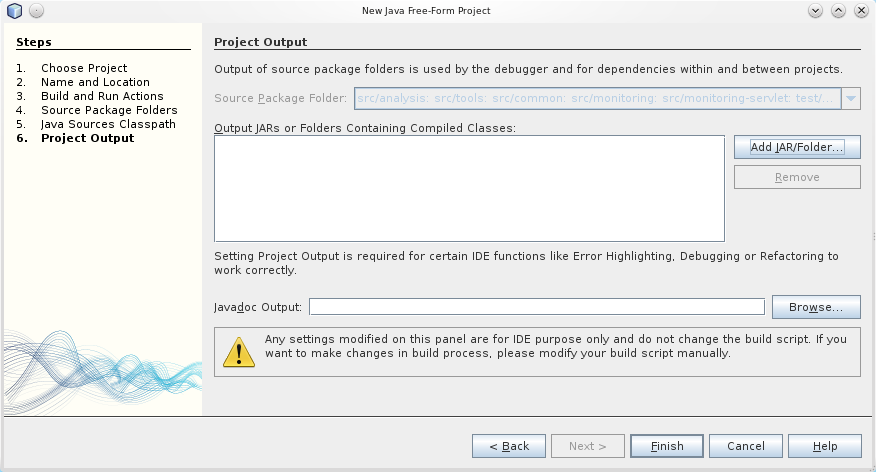
\includegraphics[scale=0.4]{figures/netbeans-ProjectOutput}
\caption{}
\label{fig:nb:projectOutput}
\end{figure}

\item Kieker should now appear in the list of projects, as shown in Fig.~\ref{fig:nb:projectTree}.  

\begin{figure}[H]\centering
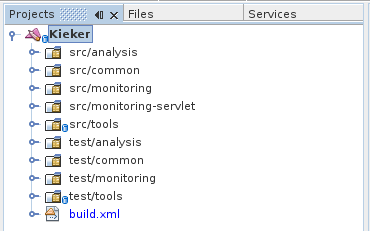
\includegraphics[scale=0.4]{figures/netbeans-ProjectTree}
\caption{}
\label{fig:nb:projectTree}
\end{figure}
\end{compactenum}
\end{compactenum}

\subsection{Eclipse}

You create an Eclipse project for the Kieker trunk as follows:

\begin{compactenum}
\item Kieker includes two sample files to create an Kieker Eclipse project: %
\begin{compactitem}
\item \texttt{eclipse-classpath.sample}
\item \texttt{eclipse-project.sample} 
\end{compactitem}

\noindent \textbf{Copy} these files to \texttt{.classpath} and \texttt{.project} respectively.

\item Open the Java project creation wizard by selecting File->New->Java Project.
\begin{compactenum}
\item \textbf{Create a Java Project (Fig.~\ref{fig:eclipse:newProject}):} %

\textbf{\underline{Un}check} \textit{Use default location} and select Kieker's %
\texttt{trunk/} directory from your filesystem. Rename the project to ``Kieker''. 

\begin{figure}[H]\centering
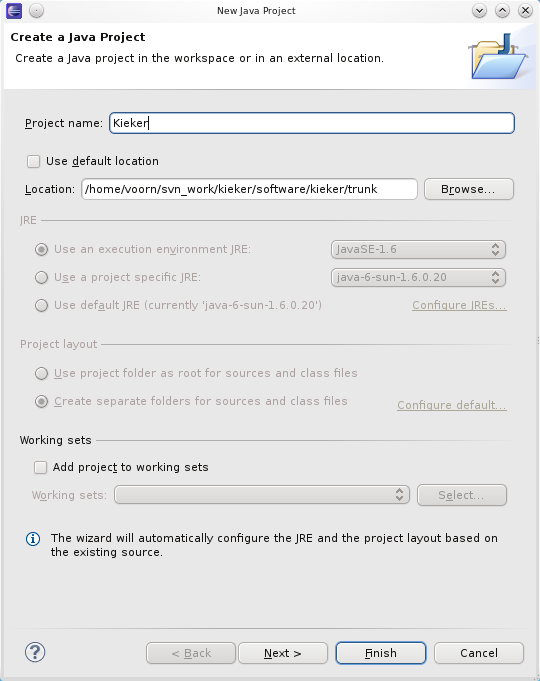
\includegraphics[scale=0.4]{figures/eclipse-NewProject}
\caption{}
\label{fig:eclipse:newProject}
\end{figure}

\item \textbf{Java Settings (Fig.~\ref{fig:eclipse:javaSettings}):} %

All settings in this dialog should be imported correctly from the \texttt{.project} %
and \texttt{.classpath} files. Simply skip this dialog without any changes and finish the wizard by clicking %
on the \textbf{Finish} button.

\begin{figure}[H]\centering
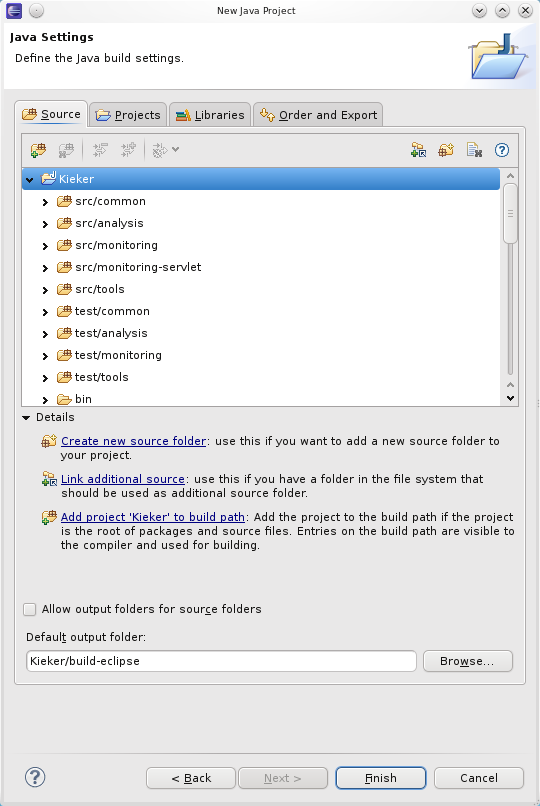
\includegraphics[scale=0.4]{figures/eclipse-JavaSettings}
\caption{}
\label{fig:eclipse:javaSettings}
\end{figure}

\item Kieker should now appear in the list of projects, as shown in Fig.~\ref{fig:eclipse:projectTree}.  

\begin{figure}[H]\centering
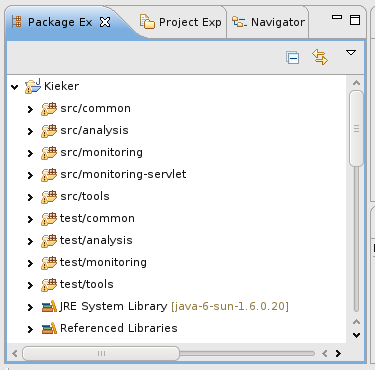
\includegraphics[scale=0.4]{figures/eclipse-ProjectTree}
\caption{}
\label{fig:eclipse:projectTree}
\end{figure}

\end{compactenum}
\end{compactenum}

\section{Continuous Integration}

Not yet performned, but we might evaluate the following tools

\begin{compactitem}
\item CruiseControl: \url{http://cruisecontrol.sourceforge.net/}
\item Hudson: \url{http://hudson-ci.org/}
\end{compactitem}


